\chapter{Дані, їх перетворення і аназіл}

У данному розділі буде описано вигляд даних, їх джерело, формат, форма, виміри та буде проведений аналіз на зв'язки та паттерни.
Також будуть описані перетворення над даними необхідні для наступного розділу.

\section{Дані}

Дані відносно викидів були взяті з офіційного сайту європейського союзу за період 2020-2023 років.
Кліматичні дані за той же період були взяті з сайту NASA. 
Ключі та відповідні назви параметрів наведені у таблиці:


\begin{center}
    \begin{tabular}{|c | c|}
        \hline
        ALLSKY SFC SW DWN & короткохвильове випромінювання неба \\
        \hline
        WD10M & напрямок вітру на висоті 10 метрів \\ 
        \hline
        WD50M & напрямок вітру на висоті 50 метрів \\
        \hline
        WS10M & швидкість вітру на висоті 10 метрів \\
        \hline
        WS50M & швидкість вітру на висоті 50 метрів  \\
        \hline
        QV2M & питома вологість на 2 метри \\
        \hline
        PS & тиск на поверхні \\
        \hline
        T2M & температура на висоті 2 метри \\
        \hline
        co conc & чадний газ, виміри $\frac{10^{-9}kg}{m^{3}}$ \\
        \hline
        no2 conc & діоксид азоту, виміри $\frac{10^{-9}kg}{m^{3}}$ \\
        \hline
        no conc & моноксид азоту, виміри $\frac{10^{-9}kg}{m^{3}}$ \\
        \hline
        o3 conc & озон, виміри $\frac{10^{-9}kg}{m^{3}}$  \\
        \hline
        pm10 conc & PM10, виміри $\frac{10^{-9}kg}{m^{3}}$ \\
        \hline
        pm2p5 conc & PM2.5, виміри $\frac{10^{-9}kg}{m^{3}}$ \\
        \hline
        so2 co & сірчастий газ, виміри $\frac{10^{-9}kg}{m^{3}}$ \\
        \hline
        time & дата замірів у форматі dd-mm-202y \\
        \hline
    \end{tabular}
    
    \vspace{1cm}
    \labelformat{2}{}{Таблиця 2.1: Розшифровка ключів з NETCDF4}
\end{center}


Формат завантажених данних - NETCDF, зберігає дані в багатовимірних масивах з прив'язкою до географічних координат та рівнів, на яких були зняті відповідні виміри. 
Географічно дані були узяті з прямокутника, координати якого - широта 44.2-52.3, довгота 30.4 - 40.3. Прямокутник яквляє собою східну частину України (див рис 2.1)


\begin{center}
    \begin{figure}[h]
        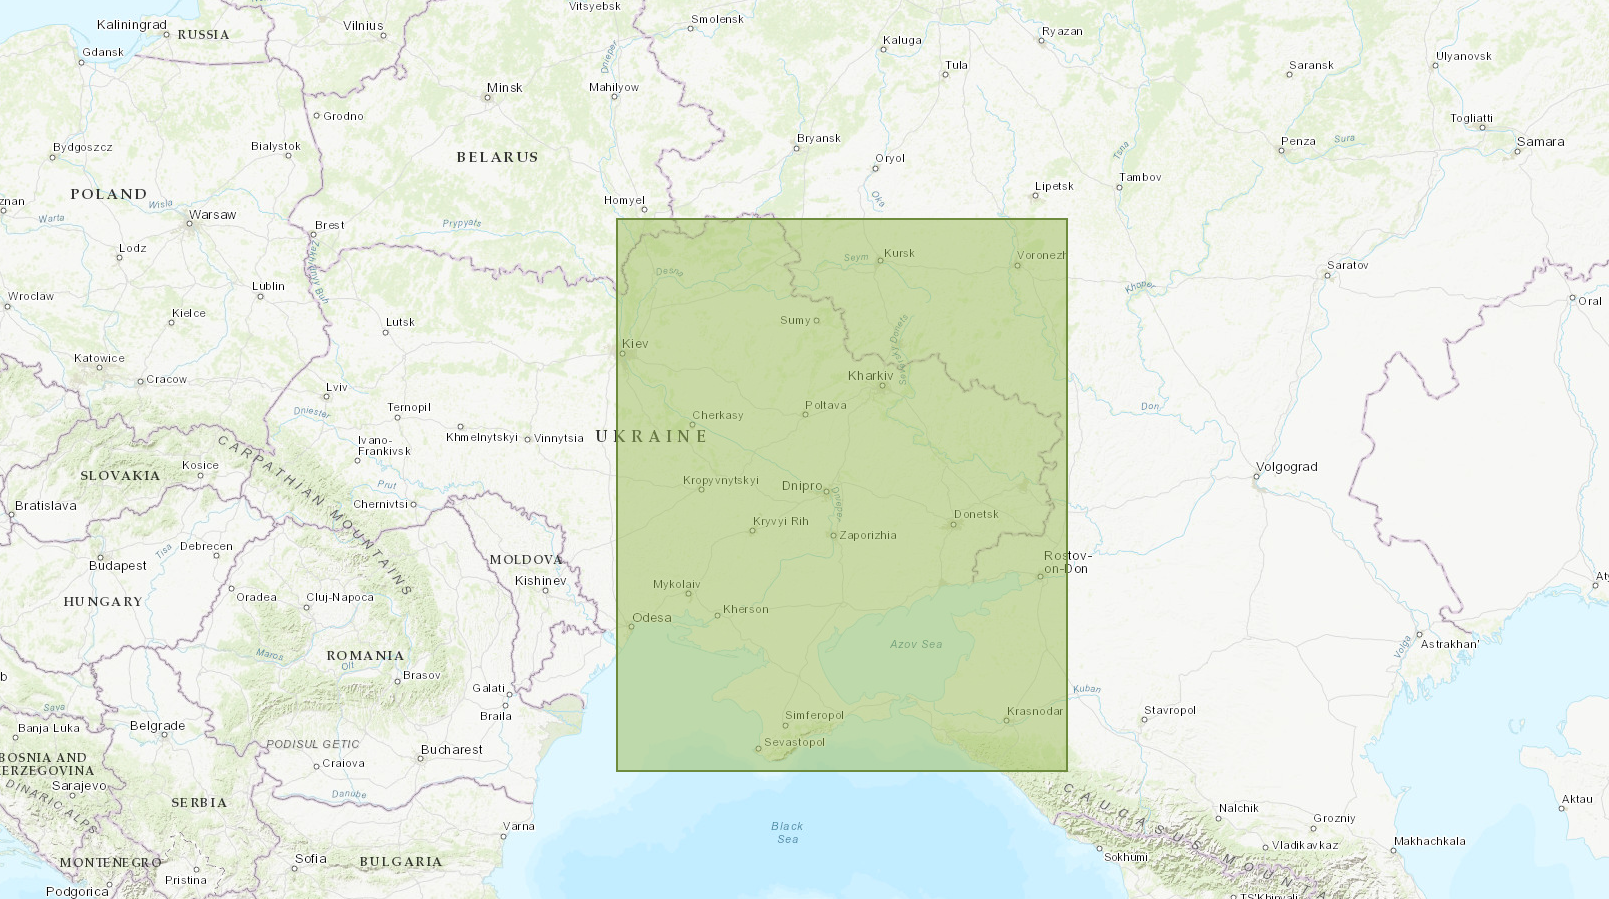
\includegraphics[width=\textwidth]{map.png}
        \caption{Мапа з прямокутником, що показує область дослідження}
    \end{figure}
\end{center}




\section{Інструменти}

Для обробки даних було використано мову програмування Python на веб-інтерактивній обчислювальній платформі Jupyter Notebook. 
Для анaлізу, ізуальзації та обробки данних були застосовані такі бібліотеки як: 

\begin{itemize}
    \item numpy - для роботи з масивами даних
    \item NETCDF4 - для роботи з NETCDF файлами
    \item matplotlib - для візуалізації даних
    \item pandas - збереження данних у форматі датафрейму і зручному використанні їх під час аналізу
    \item seaborn - аналіз даних
\end{itemize}

\section{Вигляд, паттерни та зв'язок даних}


Для ілюстрації вигляду данних про вибрані викиди, була застосована функція гістограми, що показує розподіл значень пов'язані з ними. 

\begin{center}
    \begin{figure}[h]
        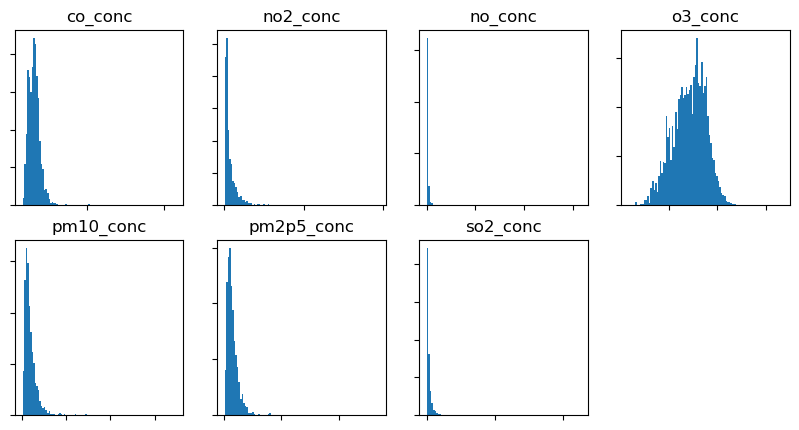
\includegraphics[width=\textwidth]{rew_data_hist.png}
        \caption{Гістограми для даних про викиди}
    \end{figure}
\end{center}

Лише дані відносно викидів озону мають розподіл подібний до нормального (за меншої кількості рівнів).
Дані відносно інших викидів утворють правосторонні розподіли.
Переважна кількість данних стосовно викидів моноксиду азоту і сірчастого газу також відповідають правосторонньому розподілу, проте через невелику кількість випадків з великою кількістю викидів на рис 2.1 цього не видно.
Для наочності наведемо діапазони усіх типів данних стосовно забруднення. 


\begin{figure}[h]
    \begin{center}
        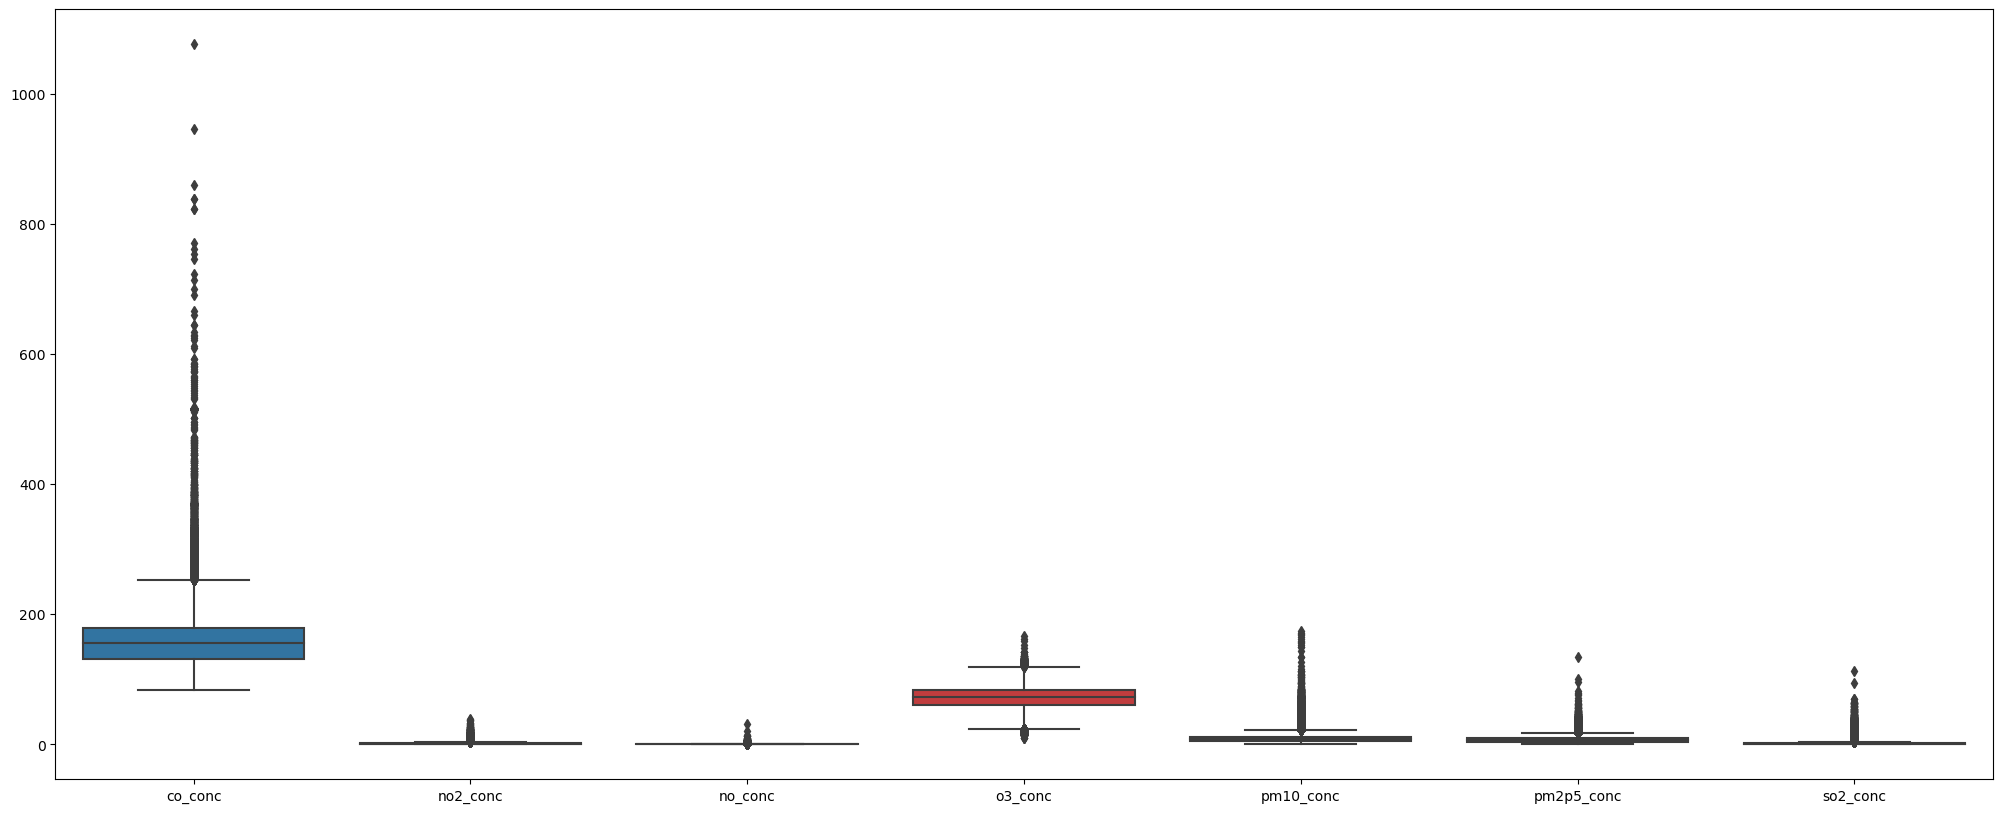
\includegraphics[width=\textwidth]{range_of_data.png}
        \caption{Діапазон даних про викиди}
    \end{center}
\end{figure}

При цьому максимуми по викидам цих типів - 31 і 112 відповідно. При цьому є лише 6 записів серед даних стосовно викидів діоксиду азоту більших за 12 і лише 2 записи відносно діоксиду сірки більших за 70.

Якщо, прибрати низькочастотні випадки отримаємо більш ілюстративні гістограми: 


\begin{center}
    \begin{figure}[h]
        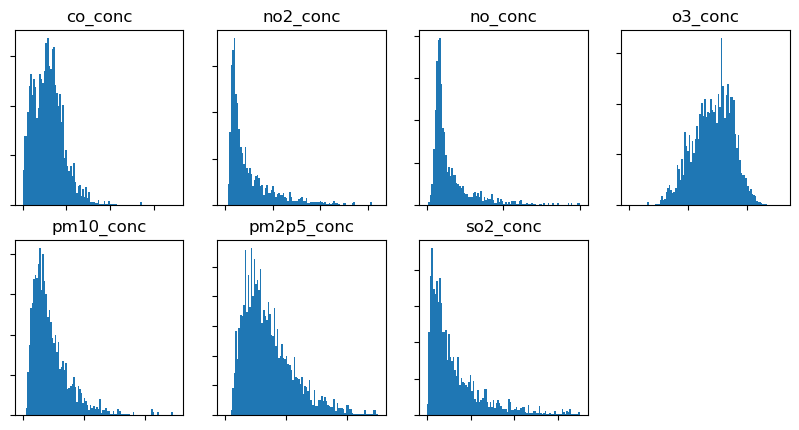
\includegraphics[width=\textwidth]{scaled_histograms.png}
        \caption{Гістограми без низьких частот для даних про викиди}
    \end{figure}
\end{center}
